%%%%%%%%%%%%%%%%%%%%%%%%%%%%% Define Article %%%%%%%%%%%%%%%%%%%%%%%%%%%%%%%%%%
\documentclass{article}
%%%%%%%%%%%%%%%%%%%%%%%%%%%%%%%%%%%%%%%%%%%%%%%%%%%%%%%%%%%%%%%%%%%%%%%%%%%%%%%

%%%%%%%%%%%%%%%%%%%%%%%%%%%%% Using Packages %%%%%%%%%%%%%%%%%%%%%%%%%%%%%%%%%%
\usepackage{geometry}
\usepackage{graphicx}
\usepackage{amssymb}
\usepackage{amsmath}
\usepackage{amsthm}
\usepackage{empheq}
\usepackage{mdframed}
\usepackage{booktabs}
\usepackage{lipsum}
\usepackage{graphicx}
\usepackage{color}
\usepackage{psfrag}
\usepackage{pgfplots}
\usepackage{bm}
%%%%%%%%%%%%%%%%%%%%%%%%%%%%%%%%%%%%%%%%%%%%%%%%%%%%%%%%%%%%%%%%%%%%%%%%%%%%%%%

% Other Settings
\usetikzlibrary{calc}

%%%%%%%%%%%%%%%%%%%%%%%%%% Page Setting %%%%%%%%%%%%%%%%%%%%%%%%%%%%%%%%%%%%%%%
\geometry{a4paper}

%%%%%%%%%%%%%%%%%%%%%%%%%% Define some useful colors %%%%%%%%%%%%%%%%%%%%%%%%%%
\definecolor{ocre}{RGB}{243,102,25}
\definecolor{mygray}{RGB}{243,243,244}
\definecolor{deepGreen}{RGB}{26,111,0}
\definecolor{shallowGreen}{RGB}{235,255,255}
\definecolor{deepBlue}{RGB}{61,124,222}
\definecolor{shallowBlue}{RGB}{235,249,255}
%%%%%%%%%%%%%%%%%%%%%%%%%%%%%%%%%%%%%%%%%%%%%%%%%%%%%%%%%%%%%%%%%%%%%%%%%%%%%%%

%%%%%%%%%%%%%%%%%%%%%%%%%% Define an orangebox command %%%%%%%%%%%%%%%%%%%%%%%%
\newcommand\orangebox[1]{\fcolorbox{ocre}{mygray}{\hspace{1em}#1\hspace{1em}}}
%%%%%%%%%%%%%%%%%%%%%%%%%%%%%%%%%%%%%%%%%%%%%%%%%%%%%%%%%%%%%%%%%%%%%%%%%%%%%%%

%%%%%%%%%%%%%%%%%%%%%%%%%%%% English Environments %%%%%%%%%%%%%%%%%%%%%%%%%%%%%
\newtheoremstyle{mytheoremstyle}{3pt}{3pt}{\normalfont}{0cm}{\rmfamily\bfseries}{}{1em}{{\color{black}\thmname{#1}~\thmnumber{#2}}\thmnote{\,--\,#3}}
\newtheoremstyle{myproblemstyle}{3pt}{3pt}{\normalfont}{0cm}{\rmfamily\bfseries}{}{1em}{{\color{black}\thmname{#1}~\thmnumber{#2}}\thmnote{\,--\,#3}}
\theoremstyle{mytheoremstyle}
\newmdtheoremenv[linewidth=1pt,backgroundcolor=shallowGreen,linecolor=deepGreen,leftmargin=0pt,innerleftmargin=20pt,innerrightmargin=20pt,]{theorem}{Theorem}[section]
\theoremstyle{mytheoremstyle}
\newmdtheoremenv[linewidth=1pt,backgroundcolor=shallowBlue,linecolor=deepBlue,leftmargin=0pt,innerleftmargin=20pt,innerrightmargin=20pt,]{definition}{Definition}[section]
\theoremstyle{myproblemstyle}
\newmdtheoremenv[linecolor=black,leftmargin=0pt,innerleftmargin=10pt,innerrightmargin=10pt,]{problem}{Problem}[section]
%%%%%%%%%%%%%%%%%%%%%%%%%%%%%%%%%%%%%%%%%%%%%%%%%%%%%%%%%%%%%%%%%%%%%%%%%%%%%%%

%%%%%%%%%%%%%%%%%%%%%%%%%%%%%%% Plotting Settings %%%%%%%%%%%%%%%%%%%%%%%%%%%%%
\usepgfplotslibrary{colorbrewer}
\pgfplotsset{width=8cm,compat=1.9}
%%%%%%%%%%%%%%%%%%%%%%%%%%%%%%%%%%%%%%%%%%%%%%%%%%%%%%%%%%%%%%%%%%%%%%%%%%%%%%%

%%%%%%%%%%%%%%%%%%%%%%%%%%%%%%% Title & Author %%%%%%%%%%%%%%%%%%%%%%%%%%%%%%%%
\title{Lines and ratios in a triangle}
\author{Jiaqi Wang \\ 1986619
\and Mil
\and Jean
\and Tom}
%%%%%%%%%%%%%%%%%%%%%%%%%%%%%%%%%%%%%%%%%%%%%%%%%%%%%%%%%%%%%%%%%%%%%%%%%%%%%%%

\begin{document}
    \maketitle
    \newpage
    \section{Problem description}
    % \section{Somthing}
    In $ \triangle ABC$ (the points $A,B,C$ are non-colinear)
    $P$ is the midpoint of the segment $BC$ and
    $R$ is the point on the line $AB$ such that $A$
    is the midpoint of the segment $BR$. Use vectors to determine the point of intersection
    $Q$ of lines $PR$ and $AC$, and show that $AQ:QC = 1:2$.

    \begin{figure}
        \label{problem drawing}
        \caption[]{figure}
        \begin{center}
            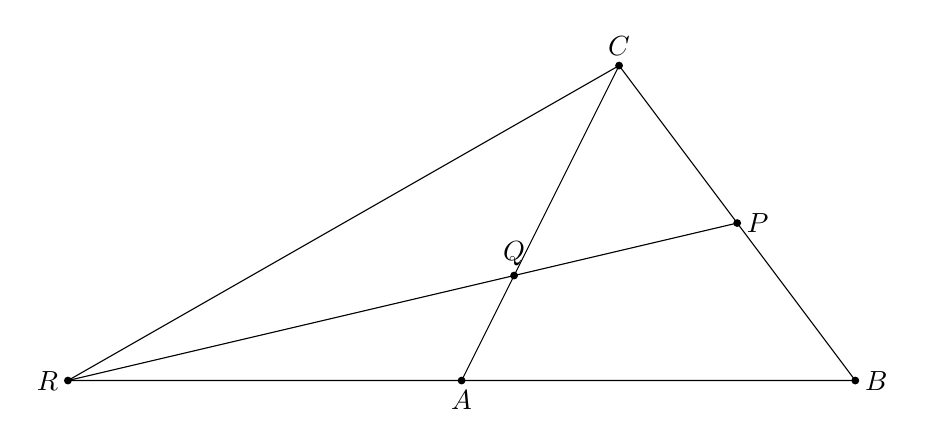
\begin{tikzpicture}
                \def\A{$A$}
                \def\B{$B$}
                \def\C{$C$}
                \def\P{$P$}
                \def\Q{$Q$}
                \def\R{$R$}
                \coordinate[label=below:\A] (A) at (0,0) ;
                \coordinate[label=right:\B] (B) at (5,0) ;
                \coordinate[label=above:\C] (C) at (2,4) ;
                \coordinate[label=right:\P] (P) at ($(B)!0.5!(C)$);
                \coordinate[label=left:\R] (R) at (-5,0);
                \coordinate[label=above:\Q] (Q) at ($(A)!1/3!(C)$);
                \draw (R) -- (A) -- (B) -- (C) -- cycle;
                \draw (A) -- (C) ;
                \draw (R) -- (P) ;
                \node[circle, fill=black, inner sep=1pt] at (A) {};
                \node[circle, fill=black, inner sep=1pt] at (B) {};
                \node[circle, fill=black, inner sep=1pt] at (C) {};
                \node[circle, fill=black, inner sep=1pt] at (P) {};
                \node[circle, fill=black, inner sep=1pt] at (R) {};
                \node[circle, fill=black, inner sep=1pt] at (Q) {};
                % \draw(0,0) node[anchor=north]{$R$}
                % -- (A)
                % -- (10,0) node[anchor=north]{$B$}
                % -- (8,4) node[anchor=south]{$C$}
                % -- cycle;
            \end{tikzpicture}
        \end{center}
    \end{figure}

    In solving the earlier described problem we will mainly use vector techniques

    \section{Solution}
    In geometric exercises that envolve vectors we need to first choose where to put the origin
    if it's not explicitly specified. We will choose point $A$ as our origin and assign vectors
    $\underbar{b}, \underbar{c}, \underbar{p}, \underbar{q}, \underbar{r}, \underbar{q}$ to the points
    $B, C, P, Q, R, Q$ respectively.


    % When solving a geometrical problem using vectors the first thing to do is to choose the origin.
    % When no constrictions are given we are free to choose any point on the plane as out origin and
    % the computations may vary in difficulty depending on our choice.
    % \par
    % In this case we can choose any of the given points as origin, or an arbitrary point $O$ as origin.





    \section{Conclusion}

    \section{Role of Homework group members}

    \section{Bibliography}
\end{document}